\documentclass[border=10pt]{standalone}
\usepackage{tikz}

\begin{document}
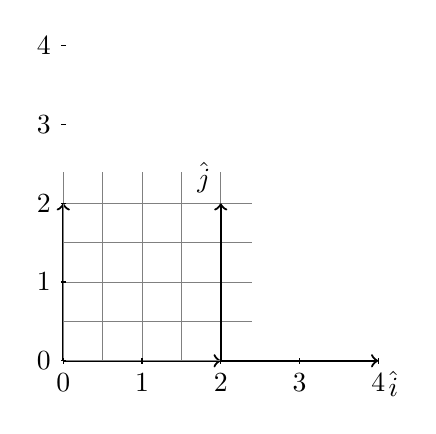
\begin{tikzpicture}[x=2cm,y=2cm] % custom unit vector lengths
\draw[thick,->] (0,0) -- (1,0);
\draw[thick,->] (0,0) -- (0,1);
\draw[step=0.5cm,gray,very thin] (0,0) grid (1.2,1.2);

\draw[thick,->] (1,0) -- (2,0) node[anchor=north west] {$\hat{i}$};
\draw[thick,->] (1,0) -- (1,1) node[anchor=south east] {$\hat{j}$};

\foreach \x in {0,1,2,3,4}
\draw (\x cm,1pt) -- (\x cm,-1pt) node[anchor=north] {$\x$};
\foreach \y in {0,1,2,3,4}
\draw (1pt,\y cm) -- (-1pt,\y cm) node[anchor=east] {$\y$};

\end{tikzpicture}
\end{document}